%%%%%%%%%%%%%%%%%%%%%%%%%%%%%%%%%%%%%%%%%
%
% Funkcionalna verifikacija hardvera
% 
%%%%%%%%%%%%%%%%%%%%%%%%%%%%%%%%%%%%%%%%%

Četvrta vežba je posvećena randomizaciji i ograničenjima. Preći će se osnovne
funkcije za randomizaciju u SystemVerilog-u, pokazati randomizacija u klasama i
osnovne konstrukcije za ograničenja. Takođe, će se pokazati kontrola random
generatora u simulatoru.\\

\emph{Constraint-driven} generisanje testova tj. generisanje testova koristeći
randomizaciju sa određenim ograničenjima umnogome olakšava automatizaciju i
pisanje testova za funkcionalnu verifikaciju. Direktno testiranje je dosta
neefikasno. Sa porastom kompleksnosti dizajna, postaje gotovo nemoguće pokriti
sve funkcionalnosti direktnim testovima. Ne samo zbog velikog broja direktnih
testova koje bi trebalo napisati, već i zbog nemogućnosti sagledanja svih
osobina dizajna i interakcije između njih. Randomizacija omogućava lak način
kreiranja testova, pokrivanje velikog broja situacija i mnogo detaljniju
verifikaciju, dok pisanje ograničenja omogućava restrikciju randomizacije na
interesantne i validne scenarije. Iako je pisanje direktnih testova u početku
lakše i brže, utrošak vremena za pisanje randomizovanog testa je opravdan jer
se, na kraju, obajvlja mnogo kvalitetnija verifikacija DUT-a.

%========================================================================================
% Section
%========================================================================================

\section{Randomizacija}

Postoji više načina za dobijanje nasumičnih vrednosti u SystemVerilog-u. Za
dobijanje pojedinačnih vrednosti postoji veliki broj ugrađenih funkcija,
međutim najveće prednosti se dobijaju koristeći random generator uz OOP.

% ----------------------------------------------------------------------------------------

\subsection{Ugrađene funkcije}

Najčešće korišćene funkcije za dobijanje nasumičnih vredosti su
\emph{\(\$\)urandom} i \emph{\(\$\)urandom\(\_\)range}. Sledi njihov opis.

\subsubsection{\emph{\(\$\)urandom}}

\emph{\(\$\)urandom} funkcija se koristi za generisanje 32-bitnog nasumičnog broja. Dobijeni broj je \emph{unsigned}, a prototip funkcije je:

\begin{lstlisting}
function int unsigned $urandom(int seed);
\end{lstlisting}
% $

\emph{seed} predstavlja opcioni argument i određuje sekvencu random brojeva
koji će biti generisani pri svakom pozivu funkcije. Pri korišćenju istog
\emph{seed}-a, random generator će uvek generisati istu sekvencu nasumičnih
brojeva. \emph{\(\$\)urandom} funckija je dosta slična \emph{\(\$\)random}
funckiji, ali vraća \emph{unsigned} brojeve i ona je stabilna za korišćenje u
nitima (\emph{threads}). Zbog toga se preporučuje korišćenje ove funkcije.

\subsubsection{\emph{\(\$\)urandom\(\_\)range}}

\emph{\(\$\)urandom\(\_\)range} funkcija vraća \emph{unsigned} integer, ali u
specificiranom opsegu. Prototip je:

\begin{lstlisting}
function int unsigned $urandom_range(int unsigned maxval, int unsigned minval = 0);
\end{lstlisting}
% $

Vraćeni broj će pripadati opsegu [maxval : minval], pri čemu je \emph{minval}
argument opcion, a podrazumevana vrednost je 0. Npr:

\begin{lstlisting}
x = $urandom_range(10, 4); // x dobija vrednost izmedju 4 i 10
x = $urandom_range(10); // x dobija vrednost izmedju 0 i 10
x = $urandom_range(4, 10); // x dobija vrednost izmedju 4 i 10, ukoliko je maxval < minval, argumenti se zamenjuju
\end{lstlisting}
% $

% ----------------------------------------------------------------------------------------

\subsection{Randomizacija i OOP}

U svakoj klasi postoji metoda \emph{randomize} koja služi za dobijanje
nasumičnih vrednosti polja.
Korišćenje klasa pruža snažan mehanizam za modelovanje podataka omogućavajući
kreiranje generičkih objekata za dobijanje nasumičnih vrednosti koji se mogu
lako ponovno koristiti, nasleđivati, uključivati/isključivati i sl.\\

Random polja u klasi se deklarišu upotrebom ključnih reči \emph{rand} i \emph{randc}. 
Ova osobina se može primeniti na bilo koji celobrojni tip, ali i na nizove i
redove.
Prilikom randomizacije nizova i redova randomizovaće se svaki element zasebno,
pri čemu je moguće ograničiti i veličinu niza (pogledati poglavlje
\ref{ssec:iter_constraints}).
Razlika između \emph{rand} i \emph{randc} modifikatora je sledeća:
\begin{itemize}
\item \emph{rand} - standardna random varijabla. Vrednosti koje prima su
  uniformno raspoređene preko čitavog opsega.
\item \emph{randc} - \emph{random-cyclic} varijabla koja iterira kroz sve
  vrednosti u datom opsegu bez ponavljanja. Maksimalna veličina promenljivih
  koje mogu biti \emph{randc} je 16 bita. Prikikom randomizacije se pronalazi
  permutacija svih mogućih vrednosti, a zatim se prilikom svakog poziva vraća
  sledeći broj u permutaciji. Nakon prolaska kroz sve elemente, pronalazi se
  sledeća nasumična permutacija.
\end{itemize}

Da bi se polja randomizovala potrebno je pozvati \emph{randomize()} metodu nad
objektom. Ako se pozove bez argumenata dodeljuje nasumičnu vrednost svim poljima
koja su deklarisana kao \emph{rand} ili \emph{randc}. Metoda vraća 1 ukoliko je
randomizacija uspešna, a 0 ukoliko nije. Korisno je uvek proveriti povratnu
vrednost pošto je lako moguće da randomizacija ne uspe ukoliko su ograničenja
pogrešno napisana i/ili postoji više ograničenja u konfliktu (ograničenja su
opisana u narednom poglavlju). Moguće je randomizovati i samo neka polja u
objektu. Ta polja se prosleđuju \emph{randomize} metodi kao argumenti. Sledi
primer randomizacije \emph{transaction} klase.

\lstinputlisting[caption=Primer \emph{randomize} metode, label=lst:randomize_example]{code/v4_randomize_example.sv}

Poziv \emph{tr.randomize()} će dodelit nasumičnu vrednost poljima \emph{addr} i
\emph{data}, dok će poziv \emph{tr.randomize(data)} randomizovati samo
\emph{data} polje, dok \emph{addr} polje ostaje nepromenjeno.\\

Provera uspešnosti randomizacije se, kao i u prethodnom primeru, često vrši
naredbom \emph{assert}. Slično kao u VHDL-u, naredba \emph{assert} proverava
izraz u zagradi i ukoliko je vrednost netačna javlja grešku.

\subsubsection{Pre i post randomize metode}

Pored \emph{randomize} metode, svaka klasa sadrži \emph{pre\(\_\)randomize} i
\emph{post\(\_\)randomize} metode, koje se automatski pozivaju pre i posle
poziva \emph{randomize} metode, respektivno. U svakoj klasi je moguće
\emph{override}-ovati ove metode kako bi se izvršile potrebne kalkulacije, ispis
vrednosti i sl.

\lstinputlisting[caption=Primer \emph{pre\(\_\)randomize} i \emph{post\(\_\)randomize} metode, label=lst:pre_post_randomize_example]{code/v4_pre_post_randomize_example.sv}

Ispis posle izvršavanja datog primera je takođe dat. Primetiti da nije potrebno
eksplicitno pozvati \emph{pre/post randomize} metode, već se njihov poziv vrši
automatski prilikom poziva \emph{randomize} metode.

% ----------------------------------------------------------------------------------------

\subsection{Std::randomize}

Iako korišćenje polja u klasi pruža velike prednosti prilikom randomizacije,
pojedini problemi ne zahtevaju veliku fleksibilnost i prednosti koje OOP pruža.
Kada je potrebno randomizovati podatak koji ne pripada klasi moguće je koristi
\emph{scope} funkciju za randomizaciju kako bi se randomizovala promenljiva u
datom opsegu bez potrebe za definisanjem klase ili instanciranjem objekta klase.
Ova funkcija je \emph{std::randomize()}.\\

Način rada ove funkcije je isti kao i klasne \emph{randomize} funkcije, s tim
što ova funkcija deluje na promenljive u trenutnom \emph{scope}-u, a ne nad
članovima klase. Primer je dat u kodu \ref{lst:std_rand}.

\lstinputlisting[caption=Primer \emph{std::randmize} metode, label=lst:std_rand]{code/v4_std_rand.sv}

Prednosti korišćenja ove funkcije, nasuprot ugrađenim \emph{\(\$\)urandom} i
\emph{\(\$\)urandom\(\_\)range}, su u mogućnosti dodavanja ograničenja
(pogledati poglavlje \ref{ssec:inline_constraints}), kao i olakšanom korišćenju
za kompleksnije promenljive.

%========================================================================================
% Section
%========================================================================================

\section{Ograničenja (engl. \emph{constraints})}

Puštanje testova sa čistim random vrednostima često nije zgodno. Trebalo bi
previše vremena da se dođe do interesantnih scenarija, možda neke vrednosti
nisu validne, možda neke nisu interesantne za proveru itd. Korišćenjem
ograničenja se mogu specificirati interesantni opsezi za generisanje
stimulusa.\\

Ograničenja se pišu u takozvanim \emph{constraint} blokovima. \emph{Constraint}
blokovi su članovi klase, kao i polja i metode, i moraju imati jedinstveno ime,
mogu se nasleđivati ili predefinisati. Blok se definiše ključnom reči
\emph{constraint} praćenom imenom ograničenja i vrednostima koje se ograničavaju
u vitičastim zagradama. Npr.

\begin{lstlisting}
constraint data_constraint { data > 5; }
\end{lstlisting}

Ograničenje pod imenom \emph{data\(\_\)constraint} ograničava vrednost
\emph{data} polja na vrednosti veće od 5, odnosno prilikom randomizacije
\emph{data} polja, uvek će mu se dodeliti nasumična vrednost veća od 5.\\

Ograničenja mogu biti i dosta kompleksnija od gore navedenog primera, i mogu
sadržati veći broj naredbi i promenljivih. Sledeći primer ograničava vrednost
\emph{addr} na 1, i vrednost \emph{data} na opseg između 5 i 10. Naredbe se
odvajanju korišćenjem ``;''.

\begin{lstlisting}
constraint addr_data_constraint { addr == 1; data > 5; data < 10;}
\end{lstlisting}

Postoji i mnogo operatora za pisanje ograničenja koji omogućavaju lako dobijanje
interesantnih vrednosti. U nastavku je dat pregled najčešće korišćenih.

% ----------------------------------------------------------------------------------------

\subsection{Pripadnost}

Koristeći \emph{inside} operator moguće je ograničiti pripadnost promenljive na
skup datih vrednosti. Sve vrednosti unutar navedenog opsega imaju jednaku
verovatnoću odabira. Npr.

\begin{lstlisting}
constraint data_inside_constraint { data inside { [8'h5 : 8'hA] }; }
\end{lstlisting}

Prethodni primer ograničava vrednost \emph{data} polja na vrednosti između 5 i
10. Obratiti pažnju na sintaksu: vrednosti koje gleda \emph{inside} operator se
navode unutar vitičastih zagrada (odvojene zarezima ukoliko ih ima više) dok se
intervali navode u uglastim zagradama. Sledeći primer dozvoljava i vrednosti 100
i 255 za \emph{data} polje:

\begin{lstlisting}
constraint data_inside_constraint { data inside { [8'h5 : 8'hA], 8'h64, 8'hFF }; }
\end{lstlisting}

Odnosno prilikom randomizacije \emph{data} polje može dobiti vrednosti iz skupa
\(\{5, 6, 7, 8, 9, 10, 100, 255\}\), sa jednakom verovatnoćom odabira svake
vrednosti.\\

Ovaj operator je moguće iskoristiti i za ograničavanje opsega kome vrednost ne
pripada, na primer:

\begin{lstlisting}
constraint data_outside_constraint { !(data inside { [8'h5 : 8'hA], 8'h64, 8'hFF }); }
\end{lstlisting}

% ----------------------------------------------------------------------------------------

\subsection{Težinska distribucija}

Ponekad je potrebno kontrolisati verovatnoću odabira pojedinih vrednosti. Ovo
omogućava \emph{dist} operator. Potrebno je operatoru proslediti listu vrednosti
i težina, odvojenih sa ``:='' ili ``:/'' operatorom. Vrednosti mogu biti
pojedinačne ili opsezi, dok su težine celobrojne vrednosti. Vrednost sa većom
težinom će biti česće dodeljivana nego vrednost sa manjom težinom. Zbir svih
težina ne mora biti jednak 100, a podrazumevana vrednost je 1.\\

``:='' operator dodeljuje težinu navedenoj vrednosti, a ukoliko je u pitanju
opseg, sve vrednosti unutar opsega će dobiti navedenu težinu. ``:/'' operator sa
druge strane će podeliti težinu sa brojem elemenata u opsegu i dodeliti tu
težinu svakoj vrednosti u opsegu, odnosno težina svake vrednosti u opsegu će
biti \textless br\(\_\)el\textgreater / \textless težina\textgreater.

\begin{lstlisting}
constraint addr_dist_constraint { addr dist {2'd0 := 5, 2'd1 := 15 }; }
\end{lstlisting}

Prethodni primer ilustruje \emph{dist} operator. Vrednosti 0 i 1 imaju težine 5
i 15, respektivno, što znači da je verovatnoća odabira vrednosti 0 za addr polje
5/20, a verovatnoća odabira vrednosti 1 je 15/20 tj. vrednost 0 će se odabrati u
25\% slučajeva, a vrednost 1 u 75\% slučajeva. U ovom primeru bismo isti
rezultat dobili i da je korišćen ``:/'' operator umesto ``:='' operatora, a
sledeći primeri ilustruju razlike između ova dva operatora:

\begin{lstlisting}
constraint addr_dist_1_constraint { addr dist {0 := 5, [1 : 3] := 15 }; }
\end{lstlisting}

Sada \emph{addr} može poprimiti vrednosti 0, 1, 2 i 3. Težina vrednosti 0 je 5,
dok svaka od vrednosti 1, 2 i 3 ima težinu 15. Ukupna težina je 5 + 3*15 = 50,
što znači da je verovatnoća odabira nule 5/50, jedinice 15/50, dvojke 15/50 i
trojke 15/50.

\begin{lstlisting}
constraint addr_dist_2_constraint { addr dist {0 :/ 5, [1 : 3] :/ 15 }; }
\end{lstlisting}

Za razliku od prethodnog primera, zbog korišćenja ``:/'' menja se način
računanja težina u intervalu. Težina vrednosti nula je i dalje 5, ali sada svaka
od vrednosti 1, 2 i 3 ima težinu 15/3 = 5. Sada je ukupna težina 20, a
verovatnoća odabira svake vrednosti 5/20.

% ----------------------------------------------------------------------------------------

\subsection{Uslovna ograničenja}

Postoji dva načina deklarisanja uslovnih ograničenja: implikacija
(\(\rightarrow\)) i \emph{if..else} konstrukcija. Npr.

\begin{lstlisting}
constraint implication_constraint { (addr == 0)-> (data == 0); }
\end{lstlisting}

Ukoliko je vrednost \emph{addr} polja nula, i vrednost \emph{data} polja se
ograničava na 0.

\begin{lstlisting}
constraint if_else_constraint {
  if(addr == 0)
    data == 0;
  else
    data == 5;
}
\end{lstlisting}

Ukoliko je \emph{addr} 0 i \emph{data} je 0, a ukoliko \emph{addr} != 0
\emph{data} je 5.
\emph{If..else} konstrukciju je zgodno koristiti ukoliko je potreban \emph{else}
deo, radi čitljivosti koda, iako se isto može postići i sa implikacijom.

% ----------------------------------------------------------------------------------------

\subsection{Iterativna ograničenja} \label{ssec:iter_constraints}

Nizove i redove je moguće ograničiti koristeći \emph{foreach} petlju i
\emph{size} metodu. Ovo se postiže na sledeći način:

\begin{lstlisting}
rand bit [7 : 0] data[$]; // queue holding 8-bit data

constraint queue_constraint{
  data.size == 5;
  foreach(data[i]) data[i] < 100;
}
\end{lstlisting}
% $

Prethodni primer ograničava red \emph{data} na tačno 5 elemenata pri čemu svaki
elemenat ima vrednost manju od 100.

% ----------------------------------------------------------------------------------------

\subsection{\emph{In-line} ograničenja} \label{ssec:inline_constraints}

Prilikom svakog poziva \emph{randomize} metode nad objektom neke klase, uzimaju
se u obzir sva ograničenja koja pripadaju toj klasi. Međutim, u nekim
slučajevima je potrebno dodati još neka ograničenja prilikom pojedinih poziva
\emph{randomize} metode. Ovo se postiže koristeći \emph{in-line} ograničenja.
Poziv \emph{randomize} metode je praćen ključnom reči \emph{with} i željenim
ograničenjima. Npr.:

\begin{lstlisting}
assert(tr.randomize() with { addr != 0; data > 2; } );
\end{lstlisting}

Primetiti da se, kao i za sva ograničenja, koriste vitičaste zagrade. Takođe,
pošto se ograničenja nalaze u opsegu klasa, dovoljno je navesti samo imena polja
\emph{addr} i \emph{data}, a ne \emph{tr.addr} i \emph{tr.data}.\\

Na isti način je moguće ograničiti \emph{std::randomize} funkciju:

\begin{lstlisting}
assert(std::randomize(x, y) with { x > y; } );
\end{lstlisting}

% ----------------------------------------------------------------------------------------

\subsection{Verovatnoće rešenja}

Tokom pisanja ograničenja važno je voditi računa o verovatnoći odabira nekog
rešenja.
Prilikom razrešavanja ograničenja mora se omogućiti uniformna distribucija nad
svim kombinacijama legalnih vrednosti promenljivih, odnosno da sve kombinacije
imaju jednaku verovatnoću odabira.
Na primer u klasi \emph{bez\(\_\)ograničenja} datoj u kodu
\ref{lst:solve_before} ne uvode se ograničenja poljima \emph{ctrl} i
\emph{data}.
Postoji 2\textsuperscript{33} mogućih rešenja i svako ima verovatnoću
1/2\textsuperscript{33} (tabela \ref{tab:unconstrained}).

\lstinputlisting[caption=Primer \emph{solve-before}, label=lst:solve_before]{code/v4_solve_before.sv}

\begin{table}[!htb]
  \centering
  \begin{tabular}{|c|c|c|}\hline
    \textbf{\emph{ctrl}}&\textbf{\emph{data}}&\textbf{Verovatnoća} \\ \hline
    0&'h00000000&1/2\textsuperscript{33} \\ \hline
    0&'h00000001&1/2\textsuperscript{33} \\ \hline
    0&'h00000002&1/2\textsuperscript{33} \\ \hline
    ...&...&... \\ \hline
    1&'hfffffffd&1/2\textsuperscript{33} \\ \hline
    1&'hfffffffe&1/2\textsuperscript{33} \\ \hline
    1&'hffffffff&1/2\textsuperscript{33} \\ \hline
  \end{tabular}
  \caption{Bez ograničenja}\label{tab:unconstrained}
\end{table}

Međutim, za neke slučajeve ovo nije željeno ponašanje.
Često su neke kombinacije od većeg interesa i treba omogućiti njihovo česće
pojavljivanje.

Na primer, ukoliko jednobitna promenljiva \emph{ctrl} kontorliše
32-bitnu promenljivu \emph{data} (kod \ref{lst:solve_before}, klasa
\emph{implikacija}) i želimo da \emph{data} ima vrednost 0 kada je \emph{ctrl}
jednak 1.
Ograničenje \emph{c\(\_\)impl} nam to omogućava.
Međutim ovo ograničenje ne znači da se prvo pronađe vrednost za \emph{ctrl}, pa
se na osnovu te vrednosti odabere vredost za \emph{data} polje.
Bez nametnutog redosleda \emph{ctrl} i \emph{data} se određuju zajedno.
Postoji ukupno 2\textsuperscript{32}+1 legalnih kombinacija vrednosti
(\emph{ctrl}, \emph{data}) koje ispunjavaju zadat uslov i sve imaju jednaku
verovatnoću odabira (tabela \ref{tab:impl}).

\begin{table}[!htb]
  \centering
  \begin{tabular}{|c|c|c|}\hline
    \textbf{\emph{ctrl}}&\textbf{\emph{data}}&\textbf{Verovatnoća} \\ \hline
    1&'h00000000&1/(2\textsuperscript{32}+1) \\ \hline
    0&'h00000000&1/(2\textsuperscript{32}+1) \\ \hline
    0&'h00000001&1/(2\textsuperscript{32}+1) \\ \hline
    0&'h00000002&1/(2\textsuperscript{32}+1) \\ \hline
    0&...& \\ \hline
    0&'hfffffffd&1/(2\textsuperscript{32}+1) \\ \hline
    0&'hfffffffe&1/(2\textsuperscript{32}+1) \\ \hline
    0&'hffffffff&1/(2\textsuperscript{32}+1) \\ \hline
  \end{tabular}
  \caption{Sa ograničenjem: implikacija}\label{tab:impl}
\end{table}

\emph{Ctrl} polje je jednako 1 samo za jednu od ovih kombinacija tj. kada je
(\emph{ctrl}, \emph{data}) = (1, 0) što znači da je verovatnoća da \emph{ctrl}
bude jednako 1 zapravo 1/(2\textsuperscript{32}+1) odnosno praktično nula, što
verovatno nije željeno ponašanje.\\

U ovom slučaju želimo da se vrednost za \emph{ctrl} bira odvojedno od
\emph{data} odnosno da se prvo razreši \emph{ctrl}, pa tek onda \emph{data}.
\emph{Solve-before} mehanizam nam ovo omogućava.
U klasi \emph{sa\(\_\)redosledom} u kodu \ref{lst:solve_before}, dodali smo
ograničenje \emph{c\(\_\)red} u kome eksplicitno navodimo da je potrebno
razrešiti polje \emph{ctrl} pre polja \emph{data}.
Navođenjem ovog ograničenja drastično menjamo verovatnoće odabira.
Sada je verovatnoća da će \emph{ctrl} polje imati vrednost 1 50\%.
Pošto \emph{data} zavisi od \emph{ctrl}, vrednost 0 će takođe biti odabrana u
blizu 50\% slučajeva.
Treba napomenuti da \emph{solve-before} mehanizam može da promeni verovatnoću
odabira vrednosti, ali ne utiče na prostor rešenja tj. na legalne kombinacije
promenljivih.
Verovatnoće za ovaj primer su prikazane u tabeli \ref{tab:solve_before}.

\begin{table}[!htb]
  \centering
  \begin{tabular}{|c|c|c|}\hline
    \textbf{\emph{ctrl}}&\textbf{\emph{data}}&\textbf{Verovatnoća} \\ \hline
    1&'h00000000&1/2 \\ \hline
    0&'h00000000&1/2 * 1/2\textsuperscript{32} \\ \hline
    0&'h00000001&1/2 * 1/2\textsuperscript{32} \\ \hline
    0&'h00000002&1/2 * 1/2\textsuperscript{32} \\ \hline
    0&...& \\ \hline
    0&'hfffffffd&1/2 * 1/2\textsuperscript{32} \\ \hline
    0&'hfffffffe&1/2 * 1/2\textsuperscript{32} \\ \hline
    0&'hffffffff&1/2 * 1/2\textsuperscript{32} \\ \hline
  \end{tabular}
  \caption{Sa ograničenjem: implikacija i \emph{solve-before}}\label{tab:solve_before}
\end{table}

% ----------------------------------------------------------------------------------------

\subsection{Kontrola}

\emph{rand\(\_\)mode()} i \emph{constraint\(\_\)mode()} metode omogućavaju
podešavanja aktivnosti promenljivih i ograničenja odnosno da li je nasumična
polje aktivno ili ne i da li je ograničenje aktivno ili ne.
U nastavku je dat njihov opis.

\subsubsection{Uključivanje i isključivanje ograničenja}

Iako se ograničenja pišu kako bi se randomizacija usmerila na scenarije od
interesa, ponekad ih je potrebno isključiti. Npr. ukoliko namerno želimo da
generišemo pogrešnu transakciju kako bi videli reakciju DUT-a. Ovo se postiže
korišćenjem metode \emph{constraint\(\_\)mode}. Metodi se kao argument
prosleđuje 0 za isključivanje ograničenja, odnosno 1 za uključivanje.
Podrazumevana vrednost je da su sva ograničenja uključena. Takođe, moguće je
isključiti/uključiti sva ograničenja ili samo neka, kao što ilustruje sledeći
primer:

\lstinputlisting[caption=Primer kontrole ograničenja, label=lst:constraint_mode_example]{code/v4_constraint_mode.sv}

\subsubsection{Uključivanje i isključivanje randomizacije}

Slčno kao i ograničenja i randomizaciju nad varijablama je moguće uključiti ili
isključiti korišćenjem metode \emph{rand\(\_\)mode}. Upotreba je ista kao i za
\emph{constraint\(\_\)mode}.

% ----------------------------------------------------------------------------------------

\subsection{Česte greške}

U ovom poglavlju je dat pregled čestih grešaka koje se prave prilikom pisanja
ograničenja, kao i preporuke za lakše korišćenje.

\begin{itemize}
\item Koristiti samo jedan odnosni operator (\textless, \textgreater , \(\geq\),
  \(\leq\), ==) unutar izraza u ograničenju. Korišćenje više može dovesti do
  neočekivanih rezultata. Npr. naredna dva primera će rezultovati različitim
  rešenjima:
  \begin{lstlisting}
constraint bad_example { 5 < a < b; }
constraint good_example { 5 < a; a < b; }
\end{lstlisting}
  Izraz u \emph{constraint} bloku se se rešava kao svi izrazi u SystemVerilog-u,
  odnosno operatori će se proveravati s leva na desno, pri čemu će rezultat biti
  jedan bit.

\item Neočekivane vrednosti se mogu javiti zbog korišćenja \emph{signed}
  promenljivih ili ukoliko se desi \emph{wrap-around}.
  \begin{lstlisting}
rand byte a, b;
constraint signed_example { a + b == 64; }
\end{lstlisting}
  U ovom primeru a i b mogu dobiti vrednosti npr. (100, -36), što možda nije
  očekivano.

\item Uvek proveriti rezultat randomizacije. Zbog velikog broja ograničenja u
  verifikacionom okruženju i mogućnosti dodavanja novih ograničenja tokom rada,
  moguće je da randomizacija neće uspeti.
  \begin{lstlisting}
if(!tr.randomize()) $error("Randomization of tr failed");
assert(tr.randomize());
\end{lstlisting}
  % $
  Takođe je moguće, posle ručne izmene vrednosti nekog polja, proveriti da li
  objekat i dalje zadovoljava sva ograničenja. Ovo se postiže prosleđivanjem
  \emph{null} vrednosti \emph{randomize} metodi. Tada se sva polja tretiraju kao
  \emph{nonrandom} i samo se proverava zadovoljivost ograničenja.
  \begin{lstlisting}
assert(tr.randomize(null));
\end{lstlisting}

\item Korišćenje istih imena u različitim \emph{scope}-ovima može dovesti do
  problema. U primeru ispod želimo da \emph{addr} polje u objektu \emph{tr}
  dobije vrednost \emph{addr} iz modula. Da bi smo to postigli potrebno je
  koristiti ``local::'' (\emph{scope resolution operator}).
  Drugi način je izbeći ponavljanje naziva, odnosno ne nazivati promenljive
  istim imenom ukoliko će se koristiti za međusobno ograničavanje.

\lstinputlisting[caption=Primer ceste greske, label=lst:same_name_constraint]{code/v4_same_name_constraint.sv}

\end{itemize}

%========================================================================================
% Section
%========================================================================================

\section{Simulacija}

Kao što je već navedeno, \emph{random seed} je broj koji služi za
inicijalizaciju pseudo-random generatora. Pri korišćenju istog \emph{seed}-a,
pseudo-random generator će uvek generisati istu sekvencu nasumičnih brojeva.
Prilikom verifikacije, uglavnom želimo da puštamo istu grupu testova sa
različitim \emph{seed}-ovima kako bismo imali veću pokrivenost. Međutim,
puštanje testova sa istim \emph{seed}-om je takođe ponekad korisno i neophodno.
Npr. ukoliko je pronađena greška koja se javlja jedino pri određenom
\emph{seed}-u (odnosno jedino pri određenoj kombinaciji nasumičnih vrednosti u
testu), potrebno je da se ona repordukuje, ali i proveri nakon ispravke.\\

Podešavanje \emph{seed}-a u Incisive Enterprise simulator-u se vrši prilikom startovanja simulacije,
prosleđivanjem \emph{sv\(\_\)seed} argumenta praćenom vrednosti \emph{seed}-a.
Ta vrednost može biti bilo koji integer ili reč \emph{random} ukoliko želimo da
se \emph{seed} nasumično odabere. Npr:

\begin{lstlisting}[language=Python]
irun top_module.sv -svseed 5
irun top_module.sv -svseed random
\end{lstlisting}

Prilikom korišćenja random \emph{seed-a}, Incisive Enterprise simulator će ispisati koja je vrednost
odabrana, kako bismo mogli da sačuvamo tu informaciju ukoliko nam bude potrebna.\\

Ukoliko se koristi simulator Vivado alata, neophodno je uraditi sledeće:
\begin{figure}[h!]
  \center
  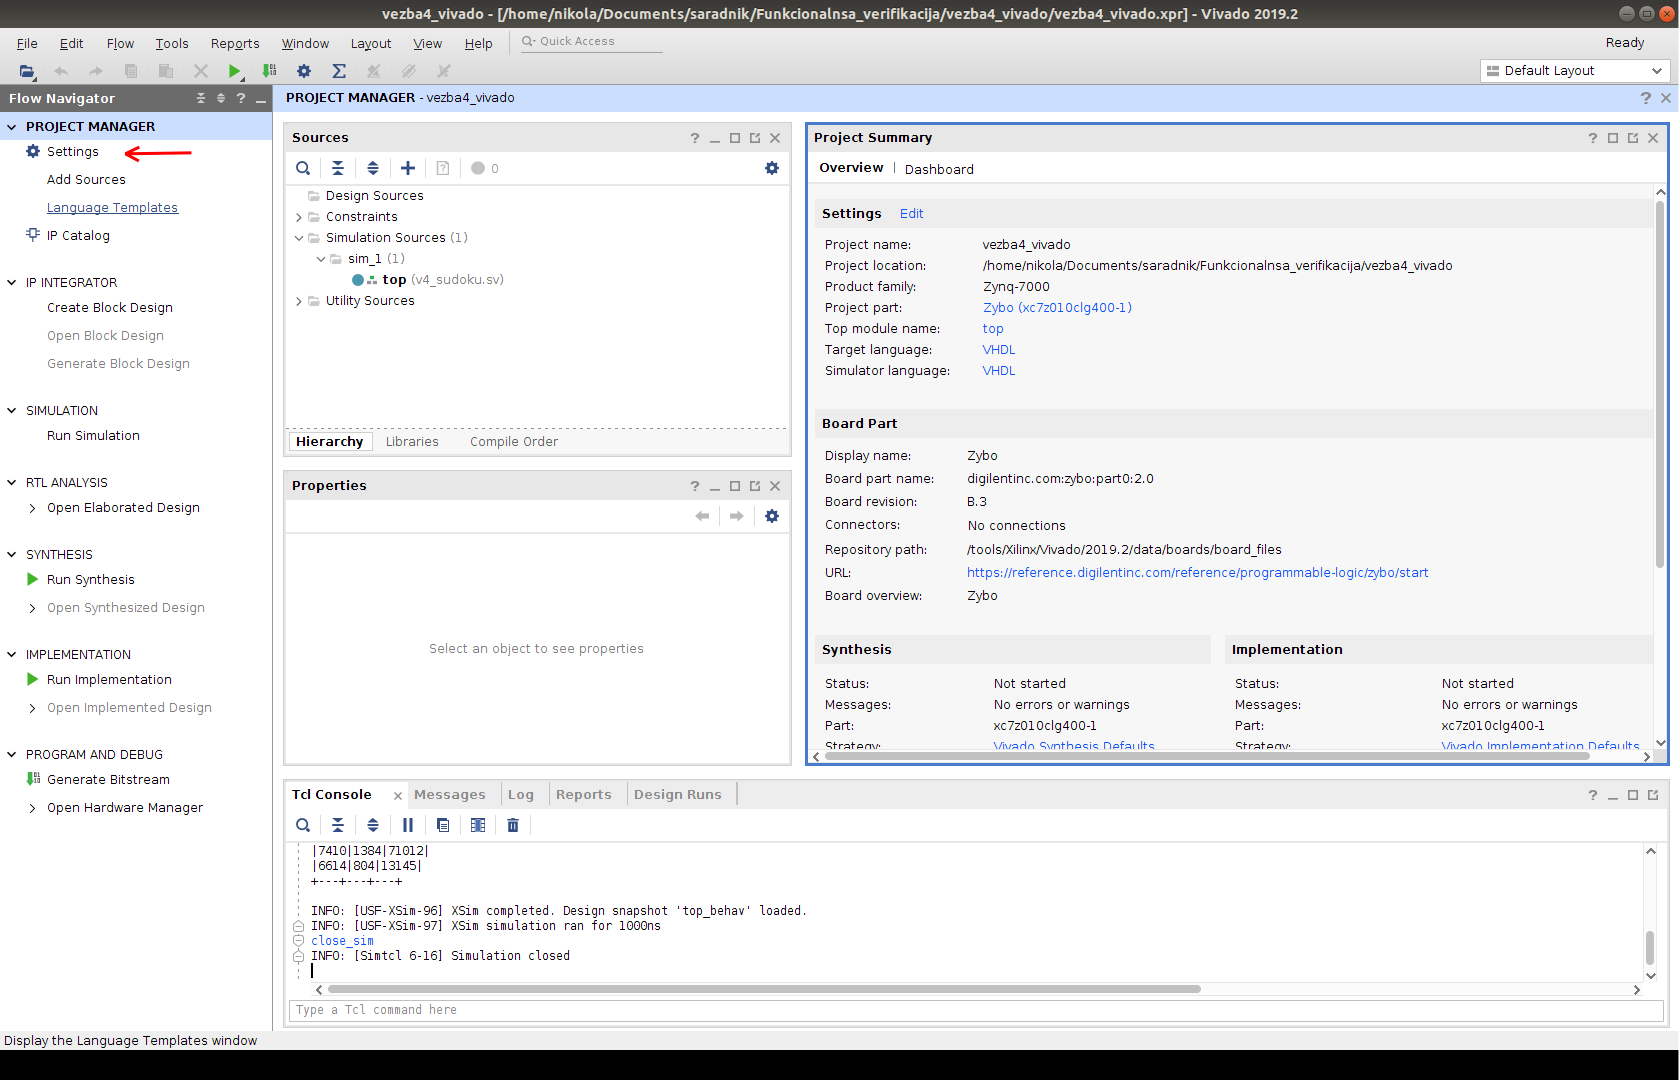
\includegraphics[width=150mm, scale=0.5]{img/v4_vivado_settings.png}
  \caption{vivado settings}
  \label{fig:vivado_settings}
\end{figure}
\newpage

Odabirom opcije settings kao što je prikazano na slici \ref{fig:vivado_settings} otvara se
prozor prikazan na slici \ref{fig:vivado_simulation_settings}

\begin{figure}[h!]
  \center
  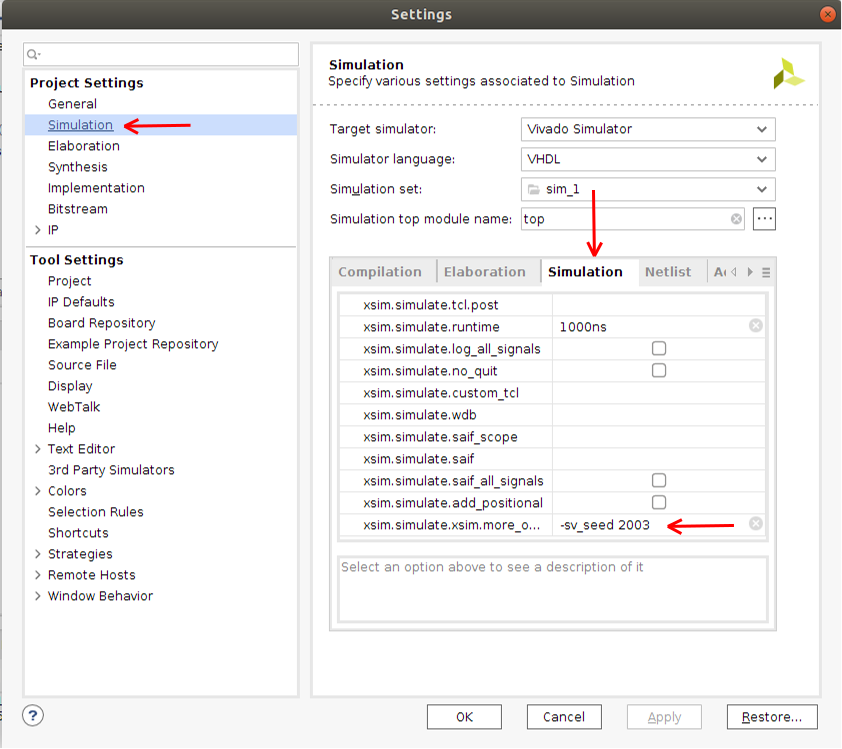
\includegraphics[width=90mm, scale=0.5]{img/v4_vivado_simulation_settings.png}
  \caption{vivado simulation settings}
  \label{fig:vivado_simulation_settings}
\end{figure}

Odabrati opcije prikazane crvenim strelicama,
i u polje \emph{xsim.simulate.xsim.more\_options} upisati:

\begin{lstlisting}[language=Python]
-sv_seed <broj_seed-a> 
\end{lstlisting}
Napomena: Ukoliko je simulacija prethodno pokrenuta, i  ponovo je izvršena promena \emph{seed-a}, neophodno je
zatvoriti simulacioni prozor i ponovo pokrenuti simulaciju.




%========================================================================================
% Section
%========================================================================================

\section{Zadaci}

\paragraph{Zadatak}

Za primer \emph{transaction} klase, ograničiti vrednost \emph{addr} polja na 2
ukoliko se \emph{data} polje nalazi u intervalu 20-50.

\paragraph{Zadatak}

Za primer \emph{transaction} klase, dodati polje \emph{read\(\_\)write} koje će
imati vrednost \emph{read} u 75\% slučajeva.

\paragraph{Zadatak}

Za primer \emph{transaction} klase, ograničiti \emph{data} polje tako da se ne
nalazi u intervalu 20-50.

\paragraph{Zadatak}

Za primer \emph{transaction} klase, dodati kontrolno polje (bit \emph{parity})
koje će predstavljati parnost \emph{data} polja i ograničiti ga na ispravne
vrednosti (odabrati \emph{even} ili \emph{odd parity}).

\paragraph{Zadatak}

Za primer \emph{transaction} klase, ukoliko je u pitanju \emph{read} transakcija
ograničiti adresu na vrednosti 0 ili 3, a \emph{data} neka dobija vrednost 0 u
12\% slučajeva, a neka je u intervalu 100-200 u 88\% slučajeva. Ukoliko je u
pitanju \emph{write} transakcija onda je vrednost podatka uvek veća od adrese i
manja od 10.

\paragraph{Zadatak}

Koristeći randomizaciju i ograničenja implementirati klasu koja služi za
rešavanje sudoku igre. Zadatak je u uneti brojeve od 1 do 9 u 9x9 mrežu tako da
se brojevi ne ponavljaju u redu, koloni ili 3x3 kvadratu. Nekoliko brojeva je
zadato unapred. Randomizovati preostala polja i napisati ograničenja tako da se
igra ispravno reši. Kod \ref{lst:sudoku} daje kostur za potrebnu klasu.

\lstinputlisting[caption=Sudoku, label=lst:sudoku]{code/v4_sudoku.sv}

%========================================================================================

